\documentclass[11pt]{article}
\usepackage{fullpage,amsthm,amsfonts,amssymb,epsfig,amsmath,times,amsthm,graphicx,wrapfig}


\begin{document}

\title{Project Writeup: Pacman Capture the Flag}
\author{Jared Jensen, Chris Gradwohl \\ Team: Organic Stupidity}
\date{CMPS 140 Winter 2017 \\ University of California, Santa Cruz}
\maketitle


\begin{abstract}
	Lorem ipsum dolor sit amet, consectetur adipiscing elit,
	sed do eiusmod tempor incididunt ut labore et dolore magna
	aliqua. Ut enim ad minim veniam, quis nostrud exercitation
	ullamco laboris nisi ut aliquip ex ea commodo consequat.
	Duis aute irure dolor in reprehenderit in voluptate velit
	esse cillum dolore eu fugiat nulla pariatur. Excepteur sint
	occaecat cupidatat non proident, sunt in culpa qui officia
	deserunt mollit anim id est laborum.
\end{abstract}


\section{Approximate Q-learning Agent}

\subsection{Fundamental Problem and Obstacles}
Our initial approach involved understanding capture the flag and determining
what type of agent would fit into this problem. We realized right away that
the game involved several strategies based on several features. It seemed like
if we could define a proper set of features then a q-learning agent would work
well in capture the flag. \

Our first goal was to create an overall offensive and defensive agent for capture the flag. We
chose to model the capture the flag problem as a set of features that the q-learning agent
could learn weights for. Initially we settled on \textit{number of food pellets, number of defending food pellets, score,
closest food pellets, opponent distance} as our set of features. These features seemed
to be working well, and once we correctly saved the weights so that all 4 agents could work together
they were performing better than expected. \

\subsection{Agent Evaluation}
In our initial implementation of the q-learning agent we did not generalize enough. We realized
that when training the agent we only did so on one map. So given the feature, the agent
was able to learn how to perform well given one map, but when it played on a random seed, it
failed miserably. \

The first problem was that we told the agent(via the feature set) to move randomly at first, and to listen to
enemy movements, while it was rewarded for obtaining food pellets.
After training on one map it was able to make its way out of the maze and into
enemy territory to obtain food pellets and receive its reward. However given a new random map,
its previous feature weights were meaningless and it was unable to get out of its initial position. \

The second problem was that we implemented the weights as a global parameter, meaning that
the agent would import and use the weights from a previous episode. This did not generalize to
a new random map.\

\subsection{Refined Approximate Q-learning Agent}
To overcome the agents mobility issues we implemented an A-star feature, that allowed
the agent to learn distances to the nearest pellet. This gave the agent the ability to
move into enemy territory in a more direct manner. \

Secondly we removed the global weights and added a weight counter to the agent object.
We did ten training games and manually added the weights the agent learned from
training. We updated the agent to have a training mode so that when training
it starts from scratch.\

With these refinements we submitted our agent to our first tournament.\

\subsection{Notable Results}
By far the most interesting(and startling) result of our q-learning agent was that
given this set of features, the agent learned how to avoid ghosts. We never actually
explicitly programed a feature that gave the agent a negative reward for being eaten.
The feature for enemy position combined with the discount rate, allowed our agent to
realize that when the \textit{opponent distance} was really low, it performed poorly.
When our agent would die it would have to go all the way to the starting part of the map, and through
learning episodes and \textit{opponent distance} feature, it found that is was bad to be
near the ghosts. In other words it obtained more rewards when it avoided
ghosts, and therefore chose actions to run away! \

This was a really cool and interesting result of feature learning. It is a great example of
choosing correct features that results in positive behavior.

% I don't know why but this has to be up here otherwise it goes to the bottom
\begin{wrapfigure}{L}{0.5\textwidth}
\centering
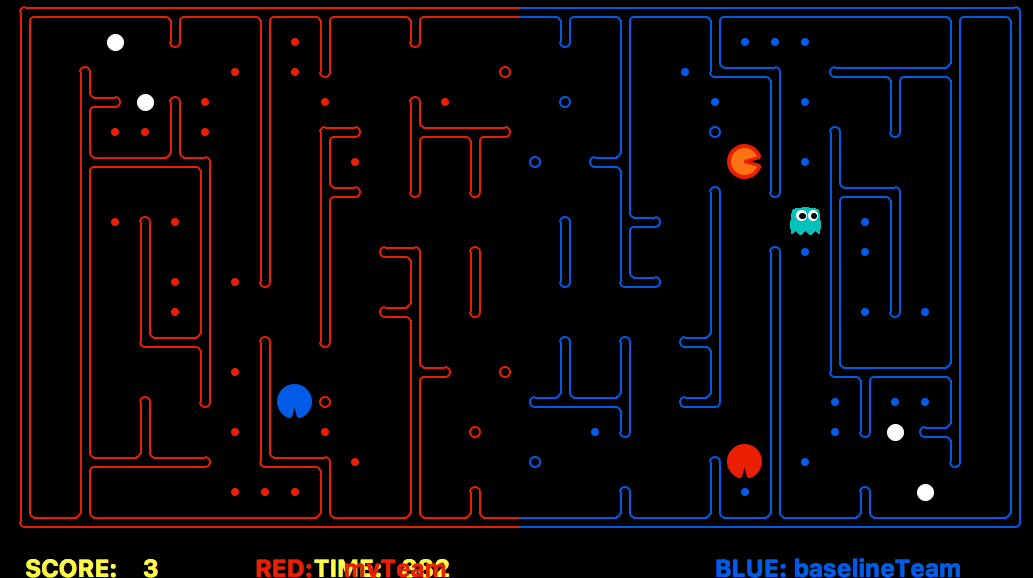
\includegraphics[width=0.5\textwidth]{report_fig1.png}
\caption{\label{fig:1}Map Bottleneck}
\end{wrapfigure}
\section{Max Flow Defense}

\subsection{Fundamental Problem and Obstacles}
With a decent offensive q-learning agent, it seemed natural to implement
a dedicated defensive agent. We needed to improve on the baseline random
action reflex agent, so we considered features that could possibly benefit
the defensive cause.By observation we noticed a unique bottleneck characteristic of
pacman levels (see teal Ghost in Figure 1). Most levels had a spot where, the ghost
could stay and completely block the enemy pacman from winning.
If we could teach our agent how to find the natural bottleneck position, then that would
prevent offense from consuming more pellets.
Therefore, our next goal became to model the game level in such a way that
allowed us to find this position given any pacman map layout.

\subsection{Model of the Problem}


We then chose to model the map as a network flow graph, and use Ford-Fulkerson
to determine the maximum flow in the graph. We constructed a framework that could
convert the map we're given into a flow network, where the vertices are the possible
non-wall positions and the edges are ordered pairs of possible positions, with two edges
(one forward and one backward) for each pair of adjacent positions. We the capacities of
all these edges to 1. We then added a source node and attached an edge with capacity
$\infty$\ to each of the vertices next to the middle line. The idea behind this was
that the enemy cound be coming from any position next to the middle line, so that's
where we would start.


Next we needed to find the bottleneck position with the most pacdots behind it in a particular game instance.
For each pacDot, we did the following:
\begin{enumerate}
	\item Find the max flow from the source to the pacDot, and the path through the maze that's returned by that max flow.
	      This flow will block any paths from the source to the given dot
	\item With the max flow still in place, for each vertex in the returned path, do the following:
	\begin{enumerate}
		\item Try to find an augmenting path through the flow using a modified version of A* from the source to the given vertex
		\item If a path exists, that means there's more than one way to get to this vertex, and we continue.\\
		      Otherwise, the vertex is being blocked by the max flow, and there is only one way to get to that vertex. Store this vertex.
	\end{enumerate}
\end{enumerate}
We then end up with a list of all of the bottlenecks for all of the pacDots.
We find the most commonly recurring bottleneck position, and that's the one we decide to go to.
We point our defense agent to that spot and tell him to stay there as long as possible\

\subsection{Agent Evaluation}
After several small modifications to Ford-Fulkerson and A* we were able
to find the bottleneck position and successfully find a path to its location.
However it became apparent that not all bottleneck locations were created equal.
That is, bottlenecks whose relative positions that were far away from the red-blue
border, were not useful to guard. If the bottleneck was far from the border, then
the defensive agent would essentially be guarding nothing or a very small amount of pellets.
Therefore we needed to find bottleneck positions that could protect a majority of
the food pellets. This did end up working very well, though, because the night we first
submitted this defense agent our ranking jumped to \#8, despite submitting a
less-than-stellar offensive agent\

\section{Final Tweaks and Manual Override}

After implementing these two ideas, our agent was running well, but there were a couple of cases where our agents
were not performing well. We decided that, instead of trying to further generalize the Q learning agents,
it would be more practical in the amount of time that we had to manually make the pacman avoid those cases.

\subsection{Eating Pacmen}
Neither of our agents netually ever decided to eat pacmen. We decided to program this in manually, so now here's what happens:
For either agent, if that agent is currently a ghost and sees a pacman close by, it considers whether to attack it.
It decides whether it should attack it based on the A* distance from that pacman and whether we're an off number of steps away.
We figured out that if a pacman was an even number of steps away from us, it was much easier for them to avoid us, so we would
ignore the pacman and continue what we previously wanted to do. For the defense agent, it also made sure that the distance between
the agent and the bottleneck it's protecting is less than the distance between the pacman and the bottleneck. This ensures that
the defense agent is always protecting the bottleneck well but still goes out and attacks pacmen, and also ensured that after
the offensive agent died, it would do a little bit of defensive work before going back on offense.

We found this strategy to help quite a bit, especially against the baseline team, because it kept their offensive agent from
getting too far into our territory most of the time.

\subsection{Avoiding ghosts}

While our Q learning agent had figured out that it should avoid ghosts by itself, it did not avoid ghosts reliably. It also often
trapped itself into corners where the ghost would easily kill it.

In order to avoid ghosts reliably, we integrated a parameter into out A* search algorithm that gave a very high weight to
all positions with ghosts in them and all positions within 2 squares of that position. This made sure that the pacman would try
to go on another route if it could find a route that avoided ghosts, and if it couldn't, then it just went on the fastest route,
hoping that the ghost moves out of its way.

In order to avoid trapping the pacman into corners, we used network flow again. If we knew a ghost was nearby, the pacman knows
it's being chased, and decides to check all nearby pacdots for one that has a maximum flow greater than 1. The idea is that if the
flow is greater than 1, there is more than one path to and from that pacdot, and so the pacman is less likely to get trapped. This\
ended up working really well and our pacman started consistently getting all of the pacdots that weren't trapped in corners very quickly.

\end{document}
